%% Template originaly created by Karol Kozioł (mail@karol-koziol.net) and modified for ShareLaTeX use

\documentclass[a4paper,13pt]{article}
\usepackage[linesnumbered,algoruled,boxed,lined]{algorithm2e}
\usepackage{multirow}
\usepackage[T1]{fontenc}
\usepackage[utf8]{inputenc}
\usepackage{graphicx}
\usepackage{xcolor}
\renewcommand\familydefault{\rmdefault}
\usepackage{tgheros}

\usepackage{amsmath,amssymb,amsthm,textcomp}
\usepackage{enumerate}
\usepackage{multicol}
\usepackage{tikz}
\usepackage[utf8]{vietnam}
\usepackage[unicode]{hyperref}
\usepackage{mathtools}
\usepackage[]{mdframed}

% draw a frame around given text
\newcommand{\framedtext}[1]{%
\par%
\noindent\fbox{%
    \parbox{\dimexpr\linewidth-2\fboxsep-2\fboxrule}{#1}%
}%
}
\newcommand\Myperm[2][^n]{\prescript{#1\mkern-2.5mu}{}P_{#2}}
\newcommand\Mycomb[2][^n]{\prescript{#1\mkern-0.5mu}{}C_{#2}}
\usepackage{geometry}
\geometry{total={210mm,297mm},
left=25mm,right=25mm,%
bindingoffset=0mm, top=22mm,bottom=25mm}

\linespread{1.3}

\newcommand{\linia}{\rule{\linewidth}{0.5pt}}

% custom theorems if needed
\newtheoremstyle{mytheor}
    {1ex}{1ex}{\normalfont}{0pt}{\scshape}{.}{1ex}
    {{\thmname{#1 }}{\thmnumber{#2}}{\thmnote{ (#3)}}}

\theoremstyle{mytheor}
\newtheorem{defi}{Definition}

% my own titles
\makeatletter
\renewcommand{\maketitle}{
\begin{center}
\vspace{2ex}
{\huge \textsc{\@title}}
\vspace{1ex}
\\
\linia\\
\@author \hfill \@date
\vspace{4ex}
\end{center}
}
\makeatother
%%%

% custom footers and headers
\usepackage{fancyhdr}
\setlength{\headheight}{20pt}
\pagestyle{fancy}
\fancyhead{} % clear all header fields
\fancyhead[L]{
 \begin{tabular}{rl}
    \begin{picture}(15,10)(0,0)
    \put(0,-8){
\includegraphics[width=8mm, height=8mm]{hcmut.png}}
    %\put(0,-8){\epsfig{width=10mm,figure=hcmut.eps}}
   \end{picture}&
	%
\includegraphics[width=8mm, height=8mm]{hcmut.png} & %
	\begin{tabular}{l}
		\textbf{\bf \ttfamily Ho Chi Minh City, University of Technology}\\
		\textbf{\bf \ttfamily Department of Computer Science and Engineer}
	\end{tabular} 	
 \end{tabular}
}
\fancyhead[R]{
	\begin{tabular}{l}
		\tiny \bf \\
		\tiny \bf 
	\end{tabular}  }
\fancyfoot{} % clear all footer fields
\fancyfoot[L]{\scriptsize \ttfamily Nghiên cứu phát triển kỹ thuật đếm số phần tử trên dòng dữ liệu}
\rfoot{Trang \thepage}
\renewcommand{\headrulewidth}{0.2pt}
\renewcommand{\footrulewidth}{0.2pt}
%

\usepackage{xcolor}
\definecolor{block-gray}{gray}{0.85}

\usepackage{environ}

\NewEnviron{myblock}
{
    \colorbox{block-gray}
    {
        \parbox{\dimexpr\linewidth-2\fboxsep\relax}
        {
            \bigbreak
            \addtolength{\leftskip}{4mm}
            \addtolength{\rightskip}{4mm}
            \BODY
        }
    }
}
\renewcommand{\quote}{\myblock}
\renewcommand{\endquote}{\endmyblock}
% code listing settings
\usepackage{listings}
\lstset{
    language=Python,
    basicstyle=\ttfamily\small,
    aboveskip={1.0\baselineskip},
    belowskip={1.0\baselineskip},
    columns=fixed,
    extendedchars=true,
    breaklines=true,
    tabsize=4,
    prebreak=\raisebox{0ex}[0ex][0ex]{\ensuremath{\hookleftarrow}},
    frame=lines,
    showtabs=false,
    showspaces=false,
    showstringspaces=false,
    keywordstyle=\color[rgb]{0.627,0.126,0.941},
    commentstyle=\color[rgb]{0.133,0.545,0.133},
    stringstyle=\color[rgb]{01,0,0},
    numbers=left,
    numberstyle=\small,
    stepnumber=1,
    numbersep=10pt,
    captionpos=t,
    escapeinside={\%*}{*)}
}
%%%----------%%%----------%%%----------%%%----------%%%

\begin{document}

\begin{titlepage}
\begin{center} {\textbf{ĐẠI HỌC QUỐC GIA TP. HỒ CHÍ MINH}
}

{\textbf{TRƯỜNG ĐẠI HỌC BÁCH KHOA}
}

{\textbf{KHOA KHOA HỌC VÀ KỸ THUẬT MÁY TÍNH }
}

{\textbf{---------------------------------------}}

\end{center}

\vspace{1cm}

\begin{figure}[h!]
\begin{center}

\includegraphics[width=3cm]{hcmut.png}
\end{center}
\end{figure}

\vspace{2cm}


\begin{center}
\textbf{\Large NGHIÊN CỨU PHÁT TRIỂN KỸ THUẬT ĐẾM SỐ PHẦN TỬ \\TRÊN DÒNG DỮ LIỆU}
\vspace{1.5cm}
\\
\textbf{\Large LUẬN VĂN THẠC SĨ}
\end{center}

\vspace{3cm}

\begin{table}[h]
\begin{tabular}{rrl}
\hspace{5.1cm} 
&\textit{Học viên: } & \textbf{LÊ ANH QUỐC}\\
&\textit{ID: } & \textbf{2070428}\\

\end{tabular}
\end{table}
\vspace{3cm}
\begin{center}
{\footnotesize HỒ CHÍ MINH CITY}
\end{center}
\end{titlepage}

\begin{titlepage}
\begin{center} {\textbf{ĐẠI HỌC QUỐC GIA TP. HỒ CHÍ MINH}
}

{\textbf{TRƯỜNG ĐẠI HỌC BÁCH KHOA}
}

{\textbf{KHOA KHOA HỌC VÀ KỸ THUẬT MÁY TÍNH }
}

{\textbf{---------------------------------------}}

\end{center}

\vspace{1cm}

\begin{figure}[h!]
\begin{center}

\includegraphics[width=3cm]{hcmut.png}
\end{center}
\end{figure}

\vspace{2cm}


\begin{center}
\textbf{\Large NGHIÊN CỨU PHÁT TRIỂN KỸ THUẬT ĐẾM SỐ PHẦN TỬ \\TRÊN DÒNG DỮ LIỆU}
\vspace{2cm}
\\
\textbf{\Large LUẬN VĂN THẠC SĨ}

\vspace{0.5cm}

\text{\small NGÀNH: KHOA HỌC MÁY TÍNH }
\vspace{0.5cm}
\\
\text{\small MÃ NGÀNH: \textbf{8480101} }
\vspace{1cm}
\\
\textbf{\small NGƯỜI HƯỚNG DẪN KHOA HỌC }
~~\\
\textbf{\small PGS. TS. THOẠI NAM}


\end{center}

\vspace{1cm}

\begin{table}[h]
\begin{tabular}{rrl}
\hspace{5.6cm} 
&\textit{Học viên: } & \textbf{lÊ ANH QUỐC}\\
&\textit{ID: } & \textbf{2070428}\\

\end{tabular}
\end{table}
\vspace{1cm}
\begin{center}
{\footnotesize HỒ CHÍ MINH CITY}
\end{center}
\end{titlepage}

%%%----------%%%----------%%%----------%%%----------%%%


%\thispagestyle{empty}

\renewcommand{\contentsname}{Content}
\newpage
\vspace{1cm}
\tableofcontents
\newpage
\section{GIỚI THIỆU ĐỀ TÀI, MỤC TIÊU VÀ ĐỐI TƯỢNG NGHIÊN CỨU}
\subsection{Tính cấp thiết và lý do chọn đề tài}
\hspace{2em}Ngày nay, các ứng dụng và dịch vụ trực tuyến đóng vai trò ngày càng quan trọng trong cuộc sống của con người. 
Chúng ta sử dụng mạng xã hội để kết nối với bạn bè và chia sẻ thông tin, mua sắm trực tuyến để tiết kiệm thời gian và tiền bạc, 
hay xem phim và chơi game trực tuyến để giải trí. Để đánh giá hiệu quả hoạt động của các ứng dụng và dịch vụ này, 
một trọng những chỉ số quan trọng nhất là số lượng người dùng hoạt động.

Việc theo dõi số lượng người dùng hoạt động trong một khoảng thời gian nhất định trên một dòng dữ liệu (data stream) 
là một yêu cầu quan trọng đối với nhiều ứng dụng và dịch vụ trực tuyến, hiệu quả của các chiến dịch marketing, 
và hỗ trợ ra quyết định kinh doanh.\\
Ví dụ, trong các ứng dụng mạng xã hội, số lượng người dùng hoạt động cho thấy mức độ tương tác 
và sự quan tâm của người dùng đối với nền tảng. Trong các dịch vụ thương mại điện tử, số lượng người dùng hoạt động cho thấy hiệu quả 
và các chiến dịch quảng cáo và khuyến mãi. \\
Tuy nhiên, việc đếm số lượng người dùng không phải là một nhiệm vụ đơn giản, đặc biệt là khi dữ liệu lớn 
và tốc độ truy cập cao. Các phương pháp truyền thống như lưu trữ và truy vấn trực tiếp vào cơ sở dữ liệu có thể gặp nhiều hạn chế về hiệu suất 
và khả năng mở rộng.\\

Trong nhiều trường hợp, cần phải tổng hợp số lượng người dùng trên nhiều dòng dữ liệu khác nhau. Việc này giúp có được bức tranh toàn cảnh về hoạt động 
của người dùng trên toàn hệ thống, từ đó đưa ra các phân tích và đánh giá chính xác hơn.\\
Ví dụ, trong hệ thống thương mại điện tử, cần tổng hợp số lượng người dùng từ các trang web, ứng dụng di động và API khác nhau để có được số lượng 
người dùng hoạt động thực tế trên toàn hệ thống. 
Tuy nhiên, việc tổng hợp dữ liệu từ nhiều nguồn khác nhau có thể gặp thách thức về đồng bộ hóa dữ liệu, xử lý dữ liệu bị thiếu hoặc lỗi, 
và đảm bảo tính nhất quán của kết quả. 

Ngoài ra, có thể cần phải đếm số lượng người dùng trên nhiều khoảng thời gian khác nhau trên một hoặc nhiều dòng dữ liệu khác nhau. 
Việc này giúp phân tích chi tiết hơn hoạt động của người dùng theo thời gian, theo khu vực hoặc theo tiêu chí khác.\\
Ví dụ, trong một ứng dụng phát trực tiếp, cần đếm số lượng người dùng hoạt động theo giờ hoặc từng phân đoạn chương trình 
để đánh giá mức độ quan tâm của người xem. Tuy nhiên, việc phân chia và xử lý dữ liệu theo nhiều đoạn có thể làm 
tăng độ phức tạp của thuật toán và ảnh hưởng đến hiệu suất của hệ thống. Do đó, cần phải có một giải pháp 
đếm số lượng phần tử trên dòng dữ liệu đạt hiệu suất cao và tin cậy, từ đó có thể ứng dụng rộng rãi trong các 
hệ thống khác nhau như mạng xã hội, thương mại điện tử, chương trình phát trực tiếp, hệ thống giám sát 
và hệ thống giao thông thông minh.

\section{CÁC CÔNG TRÌNH NGHIÊN CỨU LIÊN QUAN}
- \textbf{LogLog} - [1] \\
- \textbf{HyperLogLog} - [2]\\
- \textbf{HyperLogLog++} - [3] \\
- \textbf{Sliding HyperLogLog} - [4]\\
- \textbf{ExaLogLog} - [5] \\

\section{Phát biểu bài toán}
\subsubsection{Phát triển thuật toán để ước lượng số lượng phần tử (cardinality estimation) trên một dòng dữ liệu (data stream):}
\subsubsection{Mở rộng thuật toán để ước lượng số lượng phần tử trong một khoảng thời gian trên nhiều dòng dữ liệu:}
\subsubsection{Phát triển một thuật toán để ước lượng số lượng phần tử trên nhiều khung thời gian tỏng hợp từ nhiều dòng dữ liệu}
\section{Mục tiêu nghiên cứu}
\section{Giới hạn và đối tượng nghiên cứu }
\subsubsection{Giới hạn}
\subsubsection{Đối tượng nghiên cứu }
Đối tượng nghiên cứu của đề tài "Nghiên cứu phát triển kỹ thuật đếm số lượng phần tử trên dòng dữ liệu"

\section{HyperLogLog}
\subsection{LogLog and HyperLogLog}
Các thuật toán xác suất phổ biến nhất để ước lượng số lượng được sử dụng trong thực tế là họ các thuật toán LogLog bao gồm thuật toán \textit{LogLog}, 
được đề xuất bởi Marianne Durand và Philippe Flajolet vào năm 2003 [7], và các kế thừa của nó \textit{HyperLogLog} và \textit{HyperLogLog++}.\\
Các thuật toán này sử dụng một phương pháp tương tự như thuật toán Đếm Xác Suất trong việc ước lượng số lượng $n$ bằng cách quan sát số lượng lớn nhất 
của các số không dấu hàng đầu trong biểu diễn nhị phân của các giá trị. Tất cả chúng đều yêu cầu một bộ nhớ phụ trợ và thực hiện một lần duyệt qua dữ liệu 
để tạo ra một ước lượng về số lượng.\\
Như thường lệ, mỗi phần tử trong tập dữ liệu được tiền xử lý bằng cách áp dụng một hàm băm $h$ chuyển đổi các phần tử thành số nguyên phân bố đều đặn đủ 
trên một phạm vi scala $\{0,1,...,2^M-1\}$ hoặc, tương đương, trên tập hợp các $xâu^3$ nhị phân có độ dài M:
\[
    h(x) = j = \sum\limits_{k=0}^{M-1}j_k\cdot2^k := \left(i_0i_1...i_{M-1}\right)_2,i_k \in \{0,1\}.    
\]
\indent Các bước của các thuật toán tương tự như PCSA, chúng ta tái tạo ở đây một lần nữa. Đầu tiên, nó chia tập dữ liệu ban đầu hoặc dòng dữ liệu đầu vào 
thành một số tập con, mỗi tập con này được lập chỉ mục bởi một trong $m$ bộ đếm đơn giản. Sau đó, theo phương pháp trung bình ngẫu nhiên, vì có một 
hàm băm đơn giản, chúng ta chọn bộ đếm cho phần tử cụ thể $x$ bằng cách sử dụng một phần của giá trị băm của nó $h(x)$, trong khi phần còn lại được 
sử dụng để cập nhật bộ đếm tương ứng.\\
Tất cả các thuật toán được thảo luận ở đây dựa trên việc quan sát các mẫu $0^k1$ xuất hiện ở đầu của các giá trị cho bộ đếm cụ thể, và gán mỗi mẫu 
với chỉ số của nó, gọi là hạng. Hạng tương đương với vị trí bit 1 ít ý nghĩa nhất trong biểu diễn nhị phân của giá trị băm của phần tử được lập chỉ mục 
và có thể được tính bằng công thức (3.2). Mỗi bộ đếm đơn giản xây dựng quan sát về số lượng của riêng mình dựa trên các hạng đã nhìn thấy, ước lượng 
cuối cùng của số lượng được tạo ra từ quan sát bằng một hàm đánh giá.\\
Liên quan đến lưu trữ, các bộ đếm trong thuật toán Đếm xác suất có chi phí tương đối cao để duy trì, nhưng thuật toán \textit{LogLog} đề xuất một giải pháp 
tiết kiệm lưu trữ hơn cùng với một hàm đánh giá tốt hơn và phương pháp hiệu chỉnh sai lệch tốt hơn.
\subsection*{LogLog algorithm}
Ý tưởng cơ bản của thuật toán \textit{LogLog} bắt đầu bằng việc tính toán hạng cho mỗi phần tử đầu vào dựa trên một hàm băm đơn giản $h$. Vì chúng ta 
có thể mong đợi rằng khoảng $\frac{n}{2^k}$ phần tử có thể có $rank(\cdot) = k$, trong đó $n$ là tổng số phần tử được lập chỉ mục vào một bộ đếm, 
hạng quan sát tối đa có thể cung cấp một dấu hiệu tốt về giá trị của $log_2n$:
\[R = \underset{x \in D}{\max}\left(rank(x)\right) \approx log_2n.\]
Tuy nhiên, ước lượng như vậy có sai số khoảng $\pm1.87$ lần nhị phân, điều này không thực tế. Để giảm sai số, thuật toán \textit{LogLog} sử dụng 
một kỹ thuật phân nhóm dựa trên việc trung bình ngẫu nhiên và chia tập dữ liệu thành $m = 2^p$ tập con $S_0, S_1,..., S_{m-1}$, trong đó tham số 
độ chính xác $p$ xác định số bit được sử dụng trong điều hướng.\\
Do đó, đối với mỗi phần tử $x$ từ tập dữ liệu, $p$ bit đầu tiên của giá trị băm $h(x)$ M-bit có thể được lấy để tìm ra chỉ số $j$ của tập con thích hợp.
\[j = \left(i_0i_1...i_{p-1}\right)_2,\]
và phần còn lại (M-p) bit được lập chỉ mục vào bộ đếm tương ứng COUNTER[j] để tính hạng và nhận quan sát $R_j$ theo công thức (3.9).\\
Dưới sự phân phối công bằng, mỗi tập con nhận $\frac{n}{m}$ phần tử, do đó quan sát $R_j$ từ các bộ đếm $\{COUNTER[j]\}_{j=0}^{m-1}$ có thể cung cấp 
một dấu hiệu về giá trị của $\log_2{\frac{n}{m}}$, và bằng cách sử dụng trung bình số học của chúng với một số sự hiệu chỉnh, chúng ta có thể 
giảm thiểu phương sai của một quan sát duy nhất:
\[
    n = \alpha_m \cdot m \cdot 2 ^{\frac{1}{m}\sum\limits_{j=0}^{m-1}R_j},
\]
với $\alpha_m = \left(\Gamma\left(-\frac{1}{m}\right)\cdot \frac{1-2\frac{1}{m}}{\log_2}\right)^m$, $\Gamma(\cdot)$ là gamma function. 
Tuy nhiên, đối với hầu hết các trường hợp thực tế, $m \geq 64$ là đủ để chỉ sử dụng $\alpha_m \approx 0.39701$.\\

\begin{algorithm}[H]
    \vspace{0.25cm}
    \DontPrintSemicolon
    \LinesNumberedHidden
    \caption[]{Estimatin cardinality with \textit{LogLog}}
    \KwIn{Dataset D}
    \KwIn{Array of $m$ \textit{LogLog} counters with hash function $h$}
    \KwOut{Cardinality estimation}
    $COUNTER[j] \gets $0, $j = 0...m - 1$\\
    \For{$x \in D$}{
        $i \gets $h(x) := $(i_0i_1...i_{M-1})_2$, $i_k \in \{$0,1\}\\
        $j \gets $($i_0i_1...i_{M-1})_2$\\
        $r \gets $rank($(i_pi_{p+1}...i_{M-1})_2$)\\
        $COUNTER[j] \gets \max($COUNTER[j],r)
    }
    $R \gets \frac{1}{m} \sum\limits_{k=0}^{m-1}$COUNTER[j] \\
    \Return{$\alpha_m \cdot m \cdot 2^R$}
    \vspace{0.25cm}
\end{algorithm}
\vspace{0.25cm}
\subsection*{Properties}
Sai số tiêu chuẩn $\delta$ của thuật toán \textit{LogLog} có mối quan hệ nghịch với số lượng bộ đếm sử dụng $m$ và có thể được xấp xỉ gần như là
\[\delta \approx \frac{1.3}{\sqrt{m}}\]
\vspace{0.25cm}
\begin{quote}
    Do đó, với $m = 256$, sai số tiêu chuẩn là khoảng 8\% và với $m = 1024$, nó giảm xuống còn khoảng 4\%.
    \vspace{0.25cm}
\end{quote}
\vspace{0.25cm}
\indent Yêu cầu lưu trữ của thuật toán \textit{LogLog} có thể được ước tính là $O(log_2log_2n)$ bit nếu cần đến đếm đến $n$. Cụ thể hơn, 
tổng không gian được yêu cầu bởi thuật toán để đếm đến $n$ là $m\cdot log_2log_2\frac{n}{m}(1 + O(1))$.\\
So sánh với thuật toán Đếm Xác suất trong đó mỗi bộ đếm yêu cầu 16 hoặc 32 bit, thuật toán \textit{LogLog} yêu cầu bộ đếm nhỏ hơn 
nhiều $\{COUNTER[j]\}_{j=0}^{m-1}$, thường là 5 bit mỗi bộ đếm. Tuy nhiên, trong khi thuật toán \textit{LogLog} cung cấp hiệu quả lưu trữ tốt hơn 
so với thuật toán Đếm Xác suất, nó đôi chút ít chính xác hơn.\\

\begin{quote}
    Giả sử chúng ta cần đếm định lượng cho đến $2^{30}$, tức là khoảng 1 tỷ, với độ chính xác khoảng 4\%. Như đã đề cập, cho sai số tiêu chuẩn như vậy, 
    cần $m = 1024$ ngăn, mỗi ngăn sẽ nhận xấp xỉ $\frac{n}{m} = 2^{20}$ phần tử.\\
    $log_2\left(log_{2}2^{20}\right) \approx 4.32$, do đó, chỉ cần phân bổ khoảng 5 bit cho mỗi ngăn (tức là một giá trị nhỏ hơn 32). 
    Do đó, để ước lượng định lượng lên đến khoảng $10^9$ với sai số tiêu chuẩn là 4\%, thuật toán yêu cầu 1024 ngăn với 5 bit mỗi ngăn, 
    tức là tổng cộng 640 byte.
    \vspace{0.25cm}
\end{quote}
\vspace{0.25cm}
\subsection*{HyperLogLog algorithm}
Một cải tiến của thuật toán \textit{LogLog}, gọi là \textit{HyperLogLog}, đã được đề xuất bởi Philippe Flajolet, Eric Fusy, Olivier Gandouet và 
Frederic Meunier vào năm 2027 [9]. Thuật toán \textit{HyperLogLog} sử dụng hàm băm 32-bit, một hàm đánh giá khác nhau và các sửa lỗi bias khác nhau.\\
Tương tự như thuật toán \textit{LogLog}, \textit{HyperLogLog} sử dụng ngẫu nhiên hóa để xấp xỉ định lượng của một tập dữ liệu và đã được 
thiết kế để xử lý các định lượng lên đến $10^9$ với một hàm băm 32-bit đơn lẻ $h$ chia tập dữ liệu thành $m = 2^p$ tập con, với độ chính xác $p \in 4...16$.\\
Ngoài ra, hàm đánh giá khác biệt thuật toán \textit{HyperLogLog} so với \textit{LogLog} tiêu chuẩn. Thuật toán \textit{LogLog} gốc sử dụng 
trung bình hình học (geometric mean) trong khi \textit{HyperLogLog} sử dụng một hàm dựa trên phiên bản chuẩn hóa của trung bình điều hòa (harmonic mean):
\[
    \hat{n} \approx \alpha_m \cdot m^2 \cdot \left(\sum_{j=0}^{m-1}2^{-COUNTER[j]}\right),
\]
where
\[
    \alpha_m = \left(m\int_0^\infty\left(\log_2\left(\frac{2+x}{1+x}\right)\right)^m\text{dx}\right)^{-1}.    
\]
\indent Các giá trị xấp xỉ của $alpha_m$ có thể được tìm thấy trong Bảng 3.3.\\
Ý tưởng đằng sau việc sử dụng trung bình điều hòa là nó giảm phương sai do tính chất của nó để kiểm soát các phân phối xác suất lệch.\\
\begin{center}
    \textbf{Table 3.3:} $\alpha_m$ for most used values of $m$\\
    \begin{tabular}{ |c|c| }
        \multicolumn{2}{}{} \\ \hline
        m & $\alpha_m$ \\ \hline
        64 &  0.673 \\ \hline
        256 & 0.697 \\ \hline
        1024 & 0.709 \\ \hline
        $\ge 2^7$ & $\frac{0.7213 \cdot m}{m + 1.079}$ \\ \hline
    \end{tabular}
\end{center}

\indent Tuy nhiên, ước lượng (3.12) yêu cầu một sự điều chỉnh cho các phạm vi nhỏ và lớn do lỗi phi tuyến. Flajolet và các đồng nghiệp 
đã tìm thấy từ kinh nghiệm rằng đối với các định lượng nhỏ $n < \frac{5}{2}m$ để đạt được ước lượng tốt hơn, thuật toán \textit{HyperLogLog} 
có thể được sửa lỗi bằng Đếm Tuyến Tính bằng cách sử dụng một số bộ đếm COUNTER[j] khác không (nếu một bộ đếm có giá trị là không, 
chúng ta có thể nói chắc chắn rằng tập con cụ thể đó là trống).\\
Do đó, cho các phạm vi định lượng khác nhau, được biểu diễn dưới dạng các khoảng trên ước lượng $\hat{n}$ được tính bằng công thức (3.12), 
thuật toán cung cấp các sửa lỗi sau:
\[
    n = \left\{ \begin{array}{lcl}
        \text{LINEARCOUNTER,} & \hat{n} \leq \frac{5}{2}m \mbox{ and } \exists_j : COUNTER[j] \neq 0 \\ 
        -2^{32}\log\left(1-\frac{\hat{n}}{2^{32}}\right), & \hat{n}>\frac{1}{30}2^{32} & \mbox{\hspace{2cm}(3.13)} \\
        \hat{n}, & \textit{otherwise.}
        \end{array}\right.    
\]
\indent Tuy nhiên, đối với $n = 0$, sự sửa lỗi có vẻ không đủ và thuật toán luôn trả về một kết quả xấp xỉ $0.7m$.\\
Vì thuật toán \textit{HyperLogLog} sử dụng một hàm băm 32-bit, khi định lượng tiến gần đến $2^{32}\approx 4 \cdot 10^9$, 
hàm băm gần như đạt đến giới hạn của nó và xác suất va chạm tăng lên. Đối với các phạm vi lớn như vậy, thuật toán \textit{HyperLogLog} 
ước lượng số lượng giá trị băm khác nhau và sử dụng nó để xấp xỉ định lượng. Tuy nhiên, trong thực tế, có nguy cơ rằng một số lượng cao hơn 
không thể được đại diện và sẽ bị mất, ảnh hưởng đến độ chính xác.\\
\vspace{0.25cm}
\begin{quote}
    Xem xét một hàm băm mà ánh xạ vũ trụ thành các giá trị có độ dài M bit. Tối đa, một hàm như vậy có thể mã hóa $2^M$ 
    giá trị khác nhau và nếu định lượng ước lượng $n$ tiến dần đến giới hạn này, đụng độ hàm băm trở nên ngày càng có khả năng xảy ra.
    \vspace{0.25cm}
\end{quote}

\indent Không có bằng chứng cho thấy một số hàm băm phổ biến (ví dụ: MurmurHash3, MD5, SHA-1, SHA-256) 
hoạt động đáng kể tốt hơn các hàm khác trong các thuật toán \textit{HyperLogLog} hoặc các biến thể của nó.\\
\indent Dưới đây là toàn bộ thuật toán \textit{HyperLogLog}.\\
\begin{algorithm}[H]
    \vspace{0.25cm}
    \DontPrintSemicolon
    \LinesNumberedHidden
    \caption[]{Estimatin cardinality with \textit{HyperLogLog}}
    \KwIn{Dataset D}
    \KwIn{Array of $m$ \textit{LogLog} counters with hash function $h$}
    \KwOut{Cardinality estimation}
    $COUNTER[j] \gets $0, $j = 0...m - 1$\\
    \For{$x \in D$}{
        $i \gets $h(x) := $(i_0i_1...i_{M-1})_2$, $i_k \in \{$0,1\}\\
        $j \gets $($i_0i_1...i_{M-1})_2$\\
        $r \gets $rank($(i_pi_{p+1}...i_{M-1})_2$)\\
        $COUNTER[j] \gets \max($COUNTER[j],r)
    }
    $R \gets \frac{1}{m} \sum\limits_{k=0}^{m-1}$COUNTER[j] \\
    $\hat{n} = \alpha_m \cdot m^2 \cdot \frac{1}{R}$ \\
    $n \gets \hat{n}$ \\
    \If{$\hat{n} \le \frac{5}{2}m$}
    {
        $Z \gets \underset{j=0...m-1}{count}\left(COUNTER[j] == 0\right)$\\
        \If{$Z \ne 0$}{$n \gets m \cdot \log\left(\frac{m}{Z}\right)$}
    }
    \ElseIf{$\hat{n} > \frac{1}{30}2^{32}$}
    {
        $n \gets -2^{32}\cdot\log\left(1-\frac{n}{2^{32}}\right)$
    }
    \Return{$n$}
    \vspace{0.25cm}
\end{algorithm}
\vspace{0.25cm}
\subsection*{Properties}
Tương tự như thuật toán \textit{LogLog}, có một sự đánh đổi rõ ràng giữa sai số tiêu chuẩn $\delta$ và số lượng bộ đếm $m$:
\[\delta \approx \frac{1.04}{\sqrt{m}}.\]
\indent Yêu cầu bộ nhớ không tăng tuyến tính theo số lượng phần tử (không giống như, ví dụ, thuật toán Đếm Tuyến Tính), 
phân bổ $(M=p$) bit cho các giá trị băm và có tổng cộng $m = 2^p$ bộ đếm, bộ nhớ cần thiết là
\[\lceil\log_2\left(M + 1 - p\right)\rceil\cdot2^p \text{ bits , \indent (3.14)}\]
hơn nữa, vì thuật toán chỉ sử dụng hàm băm 32-bit và độ chính xác $p \in 4...16$, yêu cầu bộ nhớ cho 
cấu trúc dữ liệu \textit{HyperLogLog} là $5\cdot 2^p$ bit.\\
\vspace{0.4cm}
\begin{quote}
    Do đó, thuật toán \textit{HyperLogLog} cho phép ước lượng các định lượng vượt xa $10^9$ với độ chính xác thông thường là $2\%$ 
    trong khi chỉ sử dụng một bộ nhớ chỉ 1.5 KB.\\
    Ví dụ, cơ sở dữ liệu trong bộ nhớ nổi tiếng Redis duy trì cấu trúc dữ liệu \textit{HyperLogLog} của 12 KB để xấp xỉ các định lượng 
    với sai số tiêu chuẩn là 0.81.\%.
    \vspace{0.25cm}
\end{quote}

Trong khi \textit{HyperLogLog}, so với \textit{LogLog}, đã cải thiện ước lượng định lượng cho các bộ dữ liệu nhỏ, 
nó vẫn đánh giá quá cao các định lượng thực tế trong các trường hợp như vậy.\\
Các biến thể của thuật toán $HyperLogLog$ được triển khai trong các cơ sở dữ liệu nổi tiếng như Amazon Redshift, Redis, Apache CouchDB, Riak 
và các hệ thống khác.
\subsection*{HyperLogLog++ algorithm}
Sau một thời gian, vào năm 2013 [10], một phiên bản cải tiến của $HyperLogLog$ đã được phát triển, 
đó là thuật toán $HyperLogLog++$, được công bố bởi Stefan Heule, Marc Nunkesser và Alexander Hall và tập trung vào 
các định lượng lớn hơn và sửa lỗi sai tốt hơn.\\
\indent Cải tiến đáng chú ý nhất của thuật toán $HyperLogLog++$ là việc sử dụng hàm băm 64-bit. Rõ ràng, 
càng dài giá trị đầu ra của hàm băm, càng nhiều phần tử khác nhau có thể được mã hóa. Sự cải thiện này cho phép ước lượng 
các định lượng lớn hơn rất nhiều so với $10^9$ phần tử duy nhất, nhưng khi định lượng tiến gần đến $2^64 \approx 1.8\cdot 10^{19}$, 
đụng độ hàm băm cũng trở thành một vấn đề đối với $HyperLogLog++$.\\
\indent Thuật toán $HyperLogLog++$ sử dụng chính xác hàm đánh giá giống như được đưa ra trong (3.12). Tuy nhiên, nó cải thiện việc sửa lỗi sai. 
Các tác giả của thuật toán đã thực hiện một loạt các thí nghiệm để đo lường sai lệch và phát hiện rằng đối với $n \le 5m$, 
sai lệch của thuật toán $HyperLogLog$ gốc có thể được sửa lỗi hơn bằng cách sử dụng dữ liệu thực nghiệm được thu thập trong quá trình thí nghiệm.\\
\indent Ngoài bài báo gốc, Heule và đồng nghiệp cung cấp các giá trị được xác định dựa trên kinh nghiệm 
để cải thiện việc sửa lỗi sai trong thuật toán - các mảng ước lượng định lượng thô $RAWESTIMATEDATA$ và 
các sai lệch liên quan $BIASDATA$. cung cấp một mảng gồm 200 điểm nội suy, lưu trữ ước lượng thô trung bình được đo tại điểm này 
qua 5000 tập dữ liệu khác nhau. $BIASDATA$ chứa khoảng 200 sai lệch đã được đo lường tương ứng với $RAWESTIMATEDATA$. 
Cả hai mảng đều có chỉ số bắt đầu từ 0 và chứa các giá trị được tính toán trước cho tất cả các độ chính xác được hỗ trợ $p \in 4...18$,
trong đó chỉ số 0 trong các mảng tương ứng với các giá trị độ chính xác 4. Như một ví dụ, đối với $m = 2^{10} and p = 10$ 
dữ liệu cần thiết có thể được tìm thấy trong $RAWESTIMATEDATA[6]$ và $BIASDATA[6]$.\\
\indent Quy trình sửa lỗi sai trong thuật toán $HyperLogLog++$ có thể được hình thức như sau.\\
\begin{algorithm}[H]
    \vspace{0.25cm}
    \DontPrintSemicolon
    \LinesNumberedHidden
    \caption[]{Correcting bias in \textit{HyperLogLog++}}
    \KwIn{Estimate $\hat{n}$ with precicion $p$}
    \KwOut{Bias-corrected cardinality estimate}
    $n_{low} \gets 0, n_{up} \gets 0, j_{low} \gets 0, j_{up} \gets 0 $\\
    \For{$j \gets 0 to length(RAWESTIMATEDATA[p-4])$}{
        \If{$RAWESTIMATEDATA[p-4][j] \ge \hat{n}$}
        {
            $j_{low} \gets j - 1, j_{up} \gets j$\\
            $n_{low} \gets RAWESTIMATEDATA[p-4][j_{low}]$\\
            $n_{up} \gets RAWESTIMATEDATA[p-4][j_{up}]$\\
            break
        }
    }
    $b_{low} \gets BIASDATA[p-4][j_{low}]$\\
    $b_{up} \gets BIASDATA[p-4][j_{up}]$\\
    $y = interpolate\left(\left(n_{low}, n_{low} - b_{low}\right), \left(n_{up}, n_{up} - b_{up
    }\right)\right)$\\
    \Return{$y(\hat{n})$}
    \vspace{0.25cm}
\end{algorithm}
\begin{mdframed}
    \vspace{0.25cm}
    \textbf{Example 3.8: Bias correction using empirical values}\\
    Ví dụ, giả sử chúng ta đã tính toán ước lượng định lượng $\hat{n} = 2018.34$ bằng cách sử dụng công thức (3.12) và muốn sửa chúng cho 
    độ chính xác $p = 10 (m = 2^{10})$.\\
    Đầu tiên chúng ta kiểm trang mảng RAWESTIMATEDATA[6] và xác định giá trị $\hat{n}$, như vậy giá trị này rơi vào khoảng 73 đến 74,\\ với RAWESTIMATEDATA[6][73] = 2003.1804 và
    RAWESTIMATEDATA[6][74] = 2026.071.
    \[2003.1804 \le \hat{n} \le 2026.071.\]
    Ước lượng chính xác nằm trong khoảng:
    \[\left[2023.1804 - 134.1804, 2026.071 - 131.071\right] = \left[1869.0, 1895.0\right]\]
    và để tính toán ước lượng được sửa, chúng ta có thể nội suy giá trị đó, ví dụ, sử dụng tìm kiếm k-nearest neighbor hoặc chỉ là một nội suy tuyến tính\\
    $y(x) = a \cdot x + b, where y(2003.1804) = 1869.0 and y(2026.071) = 1895.0.$\\
    Do đó, bằng cách tính toán đơn giản, đường nội suy là
    \[y = 1.135837 \cdot x - 406.28725,\]
    và giá trị được nội suy cho ước lượng định lượng của chúng ta là
    \[n = y(\hat{n}) = y(2018.34) \approx 1886.218.\]
    
\end{mdframed}
\indent Theo các thí nghiệm thực hiện bởi các tác giả của HyperLogLog++, ước lượng $n_{lin}$ được tính theo thuật toán 
Linear Counting vẫn tốt hơn cho các số lượng phần tử nhỏ so với giá trị được hiệu chỉnh sai số $n$. Do đó, nếu ít nhất một bộ đếm trống tồn tại, 
thuật toán sẽ tính toán thêm ước lượng tuyến tính và sử dụng một danh sách các ngưỡng thực nghiệm, có thể tìm thấy trong Bảng 3.4, để chọn xem ước lượng 
nào nên được ưu tiên. Trong trường hợp như vậy, giá trị được hiệu chỉnh sai số $n$ chỉ được sử dụng khi ước lượng tuyến tính $n_{lin}$ 
vượt qua ngưỡng $\varkappa_m$ cho $m$ hiện tại.
\begin{mdframed}
    \vspace{0.25cm}
    \textbf{Example 3.9: Bias correction with the threshold}\\
    Trong ví dụ 3.8, khi $m = 2^{10}$, chúng ta tính được giá trị được hiệu chỉnh sai số $n \approx 1886.218$. Để xác định xem chúng ta có nên 
    ưu tiên giá trị này so với ước lượng bằng Linear Counting hay không, chúng ta cần tìm ra số lượng bộ đếm trống $Z$ trong cấu trúc dữ liệu của 
    HyperLogLog++. Vì chúng ta không có giá trị trong ví dụ của chúng ta, hãy giả định rằng $Z = 73$.\\
    Do đó, ước lượng tuyến tính theo công thức (3.1) là
    \[n_{lin} = 2^{10} \cdot \log\left(\frac{2^{10}}{73}\right) \approx 2704.\]
    Tiếp theo, chúng ta so sánh $n_{lin}$ với ngưỡng $\varkappa_m = 900$ từ Bảng 3.4, mà là rất thấp so với giá trị tính toán, do đó, 
    chúng ta ưu tiên ước lượng được hiệu chỉnh sai số $n$ so với ước lượng của Linear Counting $n_{lin}$.
    
\end{mdframed}
    
\begin{center}
    \textbf{Table 3.4: } Empirical threshold $\varkappa_m$ for the supported precision values \\
    \begin{tabular}{ |c|c|c| }
        \multicolumn{3}{}{} \\ \hline
        p & m & $\varkappa_m$ \\ \hline
        4 & $2^4$ & 10 \\ \hline
        5 & $2^5$ & 20 \\ \hline
        6 & $2^6$ & 40 \\ \hline
        7 & $2^7$ & 80 \\ \hline
        8 & $2^8$ & 220 \\ \hline
    \end{tabular}
    \hspace{0.5cm}
    \begin{tabular}{ |c|c|c| }
        \multicolumn{3}{}{} \\ \hline
        p & m & $\varkappa_m$ \\ \hline
        9 & $2^9$ & 400 \\ \hline
        10 & $2^10$ & 900 \\ \hline
        11 & $2^11$ & 1800 \\ \hline
        12 & $2^12$ & 3100 \\ \hline
        13 & $2^13$ & 6500 \\ \hline
    \end{tabular}
    \hspace{0.5cm}
    \begin{tabular}{ |c|c|c| }
        \multicolumn{3}{}{} \\ \hline
        p & m & $\varkappa_m$ \\ \hline
        14 & $2^14$ & 11500 \\ \hline
        15 & $2^15$ & 20000 \\ \hline
        16 & $2^16$ & 50000 \\ \hline
        17 & $2^17$ & 120000 \\ \hline
        18 & $2^18$ & 350000 \\ \hline
    \end{tabular}
    \hspace{0.5cm}
\end{center}

\indent The complete HyperLogLog++ algorithm is shown below.\\

\begin{algorithm}[H]
    \vspace{0.25cm}
    \DontPrintSemicolon
    \LinesNumberedHidden
    \caption[]{Estimating cardinality with \textit{HyperLogLog++}}
    \KwIn{Dataset D}
    \KwIn{Array of $m$ $LogLog$ counters with hash function $h$}
    \KwOut{Cardinality estimation}
    $COUNTER[j] \gets 0, j = 0 ... m-1$\\
    \For{$x \in D$}{
        $i \gets h(x) := (i_0i_1...i_{63})_2, i_k \in \left\{0, 1\right\}$\\
        $j \gets (i_0i_1...i_{p-1})_2$ \\
        $r \gets COUNTER[j] \gets \max(COUNTER[j], r)$
    }
    $\textbf{R} \gets \sum\limits_{k=0}^{m-1}2^{-COUNTER[j]}$\\
    $\hat{n} = \alpha_m \cdot m^2 \cdot \frac{1}{R}$\\
    $n \gets \hat{n}$\\
    \If{$\hat{n} \le 5m$}
    {
        $n \gets \textbf{CorrectBias}(\hat{n})$
    }
    $Z \gets \underset{j=0...m-1}{\textbf{count}}(COUNTER[j] = 0)$\\
    \If{$Z \ne 0$}
    {
        $n_{lin} \gets m \cdot \log\frac{m}{Z}$\\
        \If{$n_{lin} \le \varkappa_m then$}
        {
            $n \gets n_{lin}$
        }
    }
    \Return{n}
    \vspace{0.25cm}
\end{algorithm}
\subsection*{Properties}
Độ chính xác của HyperLogLog++ tốt hơn so với HyperLogLog cho một phạm vi lớn của các số lượng phần tử và tương đương tốt cho phần còn lại. 
Đối với các số lượng phần tử từ 12000 đến 61000, việc hiệu chỉnh sai số cho phép giảm thiểu sai số và tránh một đỉnh sai số khi chuyển đổi 
giữa các phụ thuộc (sub-algorithns).\\
Tuy nhiên, vì HyperLogLog++ không cần lưu trữ giá trị băm, chỉ cần một cộng với kích thước tối đa của số lượng số không đầu tiên, yêu cầu bộ nhớ 
không tăng đáng kể so với HyperLogLog và, theo (3.14), chỉ yêu cầu $6 \cdot 2^p$ bit.\\

\begin{quote}
    Thuật toán HyperLogLog++ có thể được sử dụng để ước lượng số lượng phần tử \\
    khoảng $7.9 \cdot 10^9$ với một tỷ lệ lỗi điển hình là 1.625\%, \\
    sử dụng 2.56 KB bộ nhớ.
    \vspace{0.25cm}
\end{quote}
\\\\
\indent Như đã đề cập trước đó, thuật toán sử dụng phương pháp lấy trung bình ngẫu nhiên và chia tập dữ liệu thành $m = 2^p$ tập con $\left\{COUNTER[j]\right\}_{j=0}^{m-1}$, 
mỗi bộ đếm xử lý thông tin về $\frac{n}{m}$ phần tử. Heule và đồng nghiệp đã nhận thấy rằng đối với $n \ll m$, hầu hết các bộ đếm không bao giờ được 
sử dụng và không cần phải được lưu trữ, do đó lưu trữ có thể được hưởng lợi từ một biểu diễn thưa thớt. Nếu số lượng phần tử $n$ nhỏ hơn rất nhiều 
so với $m$, thì HyperLogLog++ yêu cầu bộ nhớ đáng kể ít hơn so với các phiên bản trước đó.\\
\indent Thuật toán HyperLogLog++ trong phiên bản thưa thớt chỉ lưu trữ các cặp $(j, COUNTER[j])$, biểu diễn chúng dưới dạng một số nguyên duy nhất 
bằng cách nối các mẫu bit của chúng. Tất cả các cặp như vậy được lưu trữ trong một danh sách đã sắp xếp duy nhất của các số nguyên. 
Vì chúng ta luôn tính toán hạng cực đại, nên chúng ta không cần phải lưu trữ các cặp khác nhau có cùng chỉ số, thay vào đó chỉ cần lưu trữ cặp 
có chỉ số cực đại.
Trong thực tế, để cung cấp trải nghiệm tốt hơn, người ta có thể duy trì một danh sách không được sắp xếp khác để thực hiện các thêm nhanh 
cần phải được sắp xếp và hợp nhất định kỳ vào danh sách chính. Nếu một danh sách như vậy yêu cầu nhiều bộ nhớ hơn so với biểu diễn dày đặc 
của các bộ đếm, nó có thể dễ dàng chuyển đổi thành dạng dày đặc. Ngoài ra, để làm cho biểu diễn thưa thớt thậm chí còn thân thiện với không gian hơn, 
thuật toán HyperLogLog++ đề xuất các kỹ thuật nén khác nhau bằng cách sử dụng mã hóa độ dài biến và mã hóa sự khác biệt cho các số nguyên, 
do đó chỉ lưu trữ cặp đầu tiên và sự khác biệt từ giá trị đó.\\
\indent Hiện nay, thuật toán HyperLogLog++ được rộng rãi sử dụng trong nhiều ứng dụng phổ biến, bao gồm Google BigQuery và Elasticsearch.
\subsection*{Conclusion}
Trong chương này, chúng ta đã đi qua các phương pháp xác suất khác nhau để tính toán các phần tử duy nhất trong các tập dữ liệu lớn. 
Chúng ta đã thảo luận về những khó khăn xuất hiện trong các nhiệm vụ ước lượng số lượng phần tử và tìm hiểu về một giải pháp đơn giản có thể ước lượng 
các tập hợp có số lượng phần tử nhỏ khá tốt. Hơn nữa, chúng ta đã nghiên cứu về họ các thuật toán dựa trên việc quan sát các mẫu nhất định trong 
các biểu diễn băm của các phần tử từ tập dữ liệu, theo sau bởi nhiều cải tiến và sửa đổi đã trở thành tiêu chuẩn ngành công nghiệp ngày nay để 
ước lượng số lượng phần tử của hầu hết các loại.\\
\section{PHƯƠNG PHÁP THỰC HIỆN}
\subsubsection{Phát triển thuật toán để ước lượng số lượng phần tử (cardinality estimation) trên một dòng dữ liệu (data stream):}
TODO:
\subsubsection{Mở rộng thuật toán để ước lượng số lượng phần tử trong một khoảng thời gian trên nhiều streams:}
TODO:
\subsubsection{Phát triển một thuật toán để ước lượng số lượng phần tử trên nhiều khung thời gian tỏng hợp từ nhiều dòng dữ liệu}
TODO:

\section{KẾ HOẠCH TRIỂN KHAI}
Trong thời gian sắp tới của luận văn, tôi dự định triển khai các công việc như sau:\\
- Chuẩn bị dữ liệu, chuẩn hóa bao gồm tiền xử lý nếu có\\
- Sử dụng các mô hình học máy để hỗ trợ đánh giá SOH, SOL\\
- Tối ưu lượng thông tin lưu trữ dữ liệu và đẩy lên cloud \\
- Sử dụng các phương pháp và hiện thực mô hình \\
- Kết hợp các mô hình cloud-computing \\
- Tổng hợp kết quả và viết báo cáo\\
- Thời gian thực hiện các công việc ở biểu đồ sau:

\begin{figure}[h]
\begin{center}
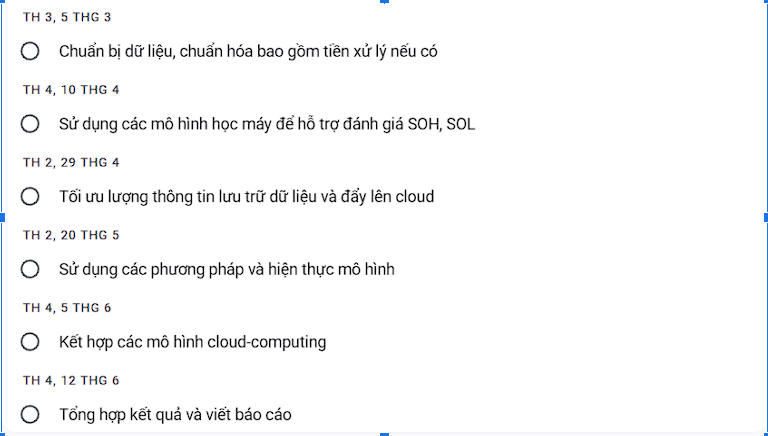
\includegraphics[width=5in]{plan.png}
\end{center}
\end{figure} 

\vspace{5cm}
\section{NỘI DUNG DỰ KIẾN CỦA LUẬN VĂN}

Nội dung báo cáo của luận văn dự kiến sẽ bao gồm các phần như sau:\\

\textbf{Chương 1: Giới thiệu}. Trong chương này sẽ trình bày một số vấn đề cơ bản của đề tài, nêu lên sự quan trọng của việc kiểm tra và giám sát thành phần trong xe điện trong lĩnh vực dữ liệu số hóa. Từ đó thấy được tầm quan trọng của đề tài để xác định rõ phạm vi và đối tượng nghiên cứu, hướng giải quyết của đề tài.
\\

\textbf{Chương 2: Các công trình nghiên cứu liên quan.} Trong chương này sẽ trình bày các công trình nghiên cứu liên quan. Tìm hiểu các phương pháp giải quyết vấn đề cũng như phạm vi, giới hạn của các nghiên cứu đó. Từ đó đánh giá tính khả thi của đề tài.\\

\textbf{Chương 3: Hiện thực và thử nghiệm mô hình. } Trong chương này sẽ trình bày chi tiết cách thức hiện thực của mô hình. Bao gồm các bước xây dựng và huấn luyện mô hình, sử dụng các mô hình và heuristic để giải quyết bài toán.\\

\textbf{Chương 4: Kết quả và đánh giá.} Trong chương này sẽ nêu ra các kết quả đạt được của mô hình, cũng như phương pháp đánh giá các kết quả đó.\\

\textbf{Chương 5: Kết luận.} Trong chương này sẽ tóm lại các ưu điểm và nhược điểm của mô hình và đưa ra các hướng nghiên cứu phát triển hệ thống trong tương lai.\\

\section{KẾT LUẬN}
Việc giám sát và quản lý pin đóng vai trò quan trọng trong đảm bảo hiệu suất, tuổi thọ và an toàn của hệ thống pin trên xe điện. Các công trình nghiên cứu liên quan đã tập trung vào các khía cạnh quan trọng như ước lượng trạng thái sạc và sức khỏe pin, chẩn đoán và tiên đoán lỗi, và quản lý thông minh của pin.\\

Để giám sát pin trên xe điện một cách hiệu quả, cần phải có hệ thống quản lý pin (BMS) thông minh và chính xác. BMS sẽ thu thập dữ liệu về trạng thái pin như trạng thái sạc, nhiệt độ, điện áp và dòng điện, sau đó phân tích và đưa ra các quyết định để bảo vệ pin và tối ưu hóa hiệu suất sử dụng năng lượng.\\

Công nghệ và phương pháp giám sát pin ngày càng phát triển, bao gồm sự kết hợp của cảm biến, hệ thống ghi dữ liệu, trí tuệ nhân tạo và học máy. Các phương pháp này giúp ước lượng trạng thái sạc và sức khỏe pin một cách chính xác, phát hiện và chẩn đoán lỗi một cách nhanh chóng, và dự đoán tuổi thọ còn lại của pin.\\

Thông qua việc nghiên cứu và áp dụng các công trình liên quan, có thể nâng cao hiệu suất và tuổi thọ của pin trên xe điện, giúp tăng khả năng di chuyển và đáp ứng nhu cầu của người sử dụng. Đồng thời, việc giám sát pin cũng đóng vai trò quan trọng trong việc đảm bảo an toàn và hạn chế các vấn đề liên quan đến pin như quá nhiệt, quá điện áp hoặc quá dòng điện.\\

Tổng quan, đề tài "Giám sát pin trên xe điện" là một lĩnh vực nghiên cứu quan trọng và đầy triển vọng, đóng góp vào sự phát triển của công nghệ pin và xe điện hiệu quả và bền vững.\\

\begin{thebibliography}{19}
    \bibitem{LogLog} M. Durand and P. Flajolet, "LogLog Counting of Large Cardinalities", Proc. European Symposium on Algorithms, 2003.
    \bibitem{HyperLogLog} P. Flajolet, E. Fusy, O. Gandouet and F. Meunier, "HyperLogLog: the analysis of a near-optimal cardinality estimation algorithm", Proceedings of the 13th conference on analysis of algorithm (AofA 07), 2007.
    \bibitem{HyperLogLog++} Hoffa, Felipe, Counting uniques faster in BigQuery with HyperLogLog++, 2017.
    \bibitem{Sliding HyperLogLog} Chabchoub, Yousra and He{\'e}brail, Georges, "Sliding hyperloglog: Estimating cardinality in a data stream over a sliding window", 2010.
    \bibitem{ExaLogLog} Ertl, Otmar, "ExaLogLog: Space-Efficient and Practical Approximate Distinct Counting up to the Exa-Scale", 2024.
    \bibitem{As87} Astrahan, M.M., Schkolnick, M., Whang, K.-Y. (1987)
    “Approximating the number of unique values of an attribute without
    sorting”, Journal Information Systems, Vol. 12 (1), pp. 11-15,
    Oxford, UK.
    
    \bibitem{Du03} Durand, M., Flajolet, P. (2003) “Loglog Counting of Large
    Cardinalities (Extended Abstract)”, In: G. Di Battista and U.
    Zwick (Eds.) - ESA 2003. Lecture Notes in Computer Science, Vol.
    2832, pp. 605-617, Springer, Heidelberg.
    
    \bibitem{Fl07} Flajolet, P., et al. (2007) “HyperLogLog: the analysis of a nearoptimal cardinality estimation algorithm”, Proceedings of the 2007
    International Conference on Analysis of Algorithms, Juan les Pins,
    France - June 17-22, 2007, pp. 127-146.
    
    \bibitem{He13} Heule, S., et al. (2013) “HyperLogLog in Practice: Algorithmic
    Engineering of a State of The Art Cardinality Estimation Algorithm”, Proceedings of the 16th International Conference on Extending
    Database Technology, Genoa, Italy —- March 18-22, 2013, pp. 683-
    692, ACM New York, NY.
    
    \bibitem{Sc07} Scheuermann, B., Mauve, M. (2007) “Near-optimal compression
    of probabilistic counting sketches for networking applications”,
    Proceedings of the 4th ACM SIGACT-SIGOPS International
    Workshop on Foundation of Mobile Computing (DIAL M-POMC),
    Portland, Oregon, USA. - August 16, 2007.
    
    \bibitem{Wh90} Whang, K.-Y., Vander-Zanden, B.T., Taylor H.M. (1990)
    “A Linear-Time Probabilistic Counting Algorithm for Database
    Applications”, Journal ACM Transactions on Database Systems,
    Vol. 15 (2), pp. 208-229.
\end{thebibliography}
\end{document}